\documentclass[dvipdfmx,autodetect-engine,titlepage]{jsarticle}
\usepackage[dvipdfm]{graphicx}
\usepackage{ascmac}
\usepackage{fancybox}
\usepackage{listings}
\usepackage{plistings}
\usepackage{itembkbx}
\usepackage{amsmath}
\usepackage{url}
\usepackage{graphics}
\usepackage{here}

\lstset{
  basicstyle={\ttfamily},
  identifierstyle={\small},
  commentstyle={\smallitshape},
  keywordstyle={\small\bfseries},
  ndkeywordstyle={\small},
  stringstyle={\small\ttfamily},
  frame={tb},
  breaklines=true,
  columns=[l]{fullflexible},
  numbers=left,
  xrightmargin=0zw,
  xleftmargin=3zw,
  numberstyle={\scriptsize},
  stepnumber=1,
  numbersep=1zw,
  lineskip=-0.5ex
}

\textheight=23cm
\renewcommand{\figurename}{図}
\renewcommand{\tablename}{表}
\newenvironment{code}
{\vspace{0.5zw}\VerbatimEnvironment  \begin{screen} 
\baselineskip=1.0\normalbaselineskip
 \begin{Verbatim}}
{\end{Verbatim}
\baselineskip=\normalbaselineskip
 \end{screen}\vspace{0.5zw}} 

\title{ビッグデータ解析(A1)\\
第4回レポート\\
}
\author{2600200087-2\\Oku Wakana\\奥 若菜}
\date{Jan.22 2023}

\begin{document}

\maketitle

\section{既習手法の技術マップ}

1.重回帰分析  2.判別分析  3.主成分分析  4.多次元尺度法\\
 5.数量化I類  6.数量化II類  7.数量化IV類

\section{主成分分析}
\subsection{第2主成分までで2次元平面にプロットせよ}

\begin{figure}[H]
  \centering
  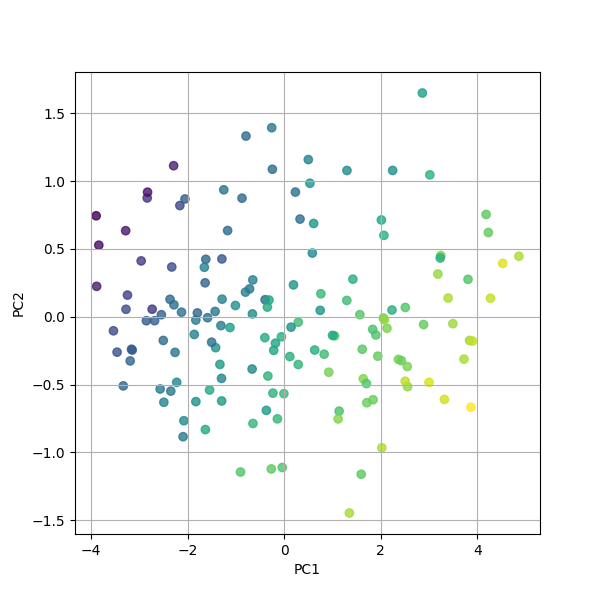
\includegraphics[scale=0.5]{CPA.png}
  \caption{主成分得点}\label{fig:図1}
\end{figure}

\subsection{第6主成分までの累積寄与率をグラフに示せ}

\begin{figure}[H]
  \centering
  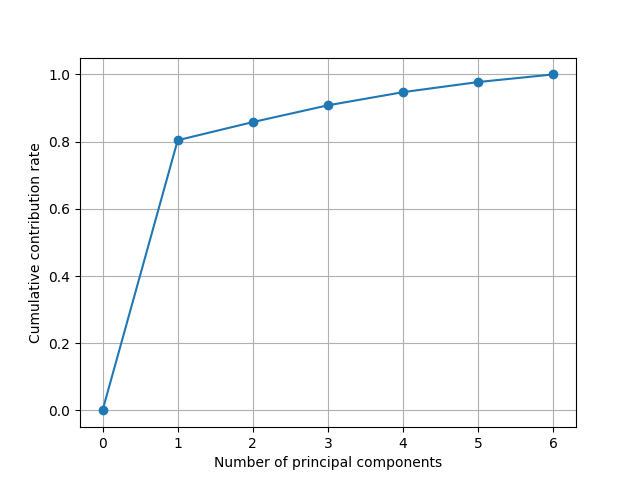
\includegraphics[scale=0.5]{ccr.png}
  \caption{累積寄与率}\label{fig:図2}
\end{figure}

\subsection{6つの主成分について,6項目の特徴の主成分負荷量を求め,各主成分がどのような意味をもつのかを解釈せよ.}

\begin{table}[H]
  \centering
  \begin{tabular}{|c|c|c|c|c|c|c|}
  \hline
      & 図書館蔵書   & 教室の多さ   & 女子学生の比率 & 教員の多さ   & 学生の多さ   & 博士課程学生の多さ \\ \hline
  PC1 & 0.3975  & 0.4178  & 0.4105  & 0.4171  & 0.3985  & 0.4073    \\ \hline
  PC2 & -0.7326 & -0.2131 & 0.3734  & 0.3342  & 0.3778  & -0.1546   \\ \hline
  PC3 & -0.2793 & -0.0038 & 0.3853  & -0.0243 & -0.6702 & 0.5689    \\ \hline
  PC4 & 0.1649  & -0.5931 & 0.2080  & -0.5220 & 0.3981  & 0.3828    \\ \hline
  PC5 & 0.3818  & -0.2135 & 0.6503  & 0.0098  & -0.2620 & -0.5628   \\ \hline
  PC6 & 0.2327  & -0.6184 & -0.2778 & 0.6640  & -0.1481 & 0.1521    \\ \hline
  \end{tabular}
  \end{table}

  \begin{itemize}
    \item  \textgt{第1主成分}\\
    すべて変数係数が正で互いに強め合っている.第1主成分が総合点であることをよく示している.
    \item  \textgt{第2主成分}\\
    女子学生の比率や教員の多さ,学生の多さが正,図書館蔵書や教室の多さが負になっている.人の充実度vs施設の充実度の軸であると言える.
    \item \textgt{第3主成分}\\
    博士課程学生の多さが大きく正となり,女子学生の比率も正となっている.一方で学生の多さは大きく負になっており,少人数に研究のリソースを当てることが重視されていると言える.
    \item \textgt{第4主成分}\\
    教室の多さと教員の多さが大きく負となっており,学生の多さや博士課程学生の多さは正となっている.
    教育の充実度vs学生の多さの軸になっていると言える.
    \item \textgt{第5主成分}\\
    女子学生の多さが大きく正,博士課程学生の多さが大きく負となっており,女子学生の多さvs博士課程学生の多さの軸になっていると言える.
    \item \textgt{第6主成分}\\
    教員の多さが大きく正,教室の多さが大きく負となっており,教員の多さvs教室の多さの軸になっていると言える.\\\\
\end{itemize}

\textgt{以下プログラムのソースコードを示す.}\\

\begin{lstlisting}[caption=pythonプログラム,label=1]
import numpy as np
import pandas as pd
from pandas import plotting 
import urllib.request 
import matplotlib.pyplot as plt
import sklearn #機械学習のライブラリ
from sklearn.decomposition import PCA #主成分分析器
import csv

df = pd.read_csv("univ-power.csv")
print(df.head())

# 行列の標準化
# dfs = df.iloc[:, 1:].apply(lambda x: (x-x.mean())/x.std(), axis=0)
dfs = (df - df.mean()) / df.std(ddof=0)
print(dfs.head())

#主成分分析の実行
pca = PCA()
pca.fit(dfs)

# データを主成分空間に写像
feature = pca.transform(dfs)

# 主成分得点
pd.DataFrame(feature, columns=["PC{}".format(x + 1) for x in range(len(dfs.columns))]).head()
print(feature)

#第一主成分と第二主成分でプロットする
plt.figure(figsize=(6, 6))
plt.scatter(feature[:, 0], feature[:, 1], alpha=0.8, c=list(dfs.iloc[:, 0]))
plt.grid()
plt.xlabel("PC1")
plt.ylabel("PC2")
plt.show()

# 寄与率
pd.DataFrame(pca.explained_variance_ratio_, index=["PC{}".format(x + 1) for x in range(len(dfs.columns))])
print(pca.explained_variance_ratio_)

# 累積寄与率を図示する
import matplotlib.ticker as ticker
plt.gca().get_xaxis().set_major_locator(ticker.MaxNLocator(integer=True))
plt.plot([0] + list( np.cumsum(pca.explained_variance_ratio_)), "-o")
plt.xlabel("Number of principal components")
plt.ylabel("Cumulative contribution rate")
plt.grid()
plt.show()

# PCA の固有値
print(pd.DataFrame(pca.explained_variance_, index=["PC{}".format(x + 1) for x in range(len(dfs.columns))]))

# PCA の固有ベクトル
print(pca.components_)
# pd.DataFrame(pca.components_, columns=df.columns[1:], index=["PC{}".format(x + 1) for x in range(len(dfs.columns))])


\end{lstlisting}

\end{document}